
\begin{figure}[h] 
\caption{Average precision for all white lists}
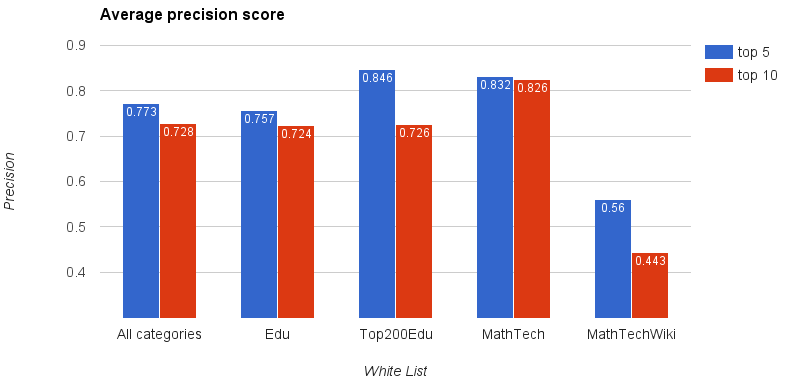
\includegraphics[width=\textwidth]{charts/avgPrecision}
\label{fig:avgPrecision}
\end{figure}

\begin{figure}[h] 
\caption{Precision score when the keyword \textit{Logic} is used as a search phrase, with the different white lists applied.}
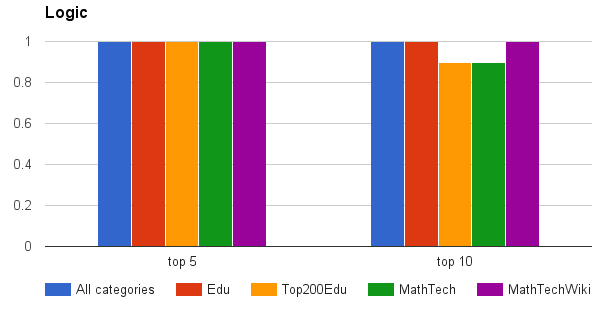
\includegraphics[width=\textwidth]{charts/l}
\label{fig:l}
\end{figure}

\begin{figure}[h] 
\caption{Precision score when the keyword \textit{Programming} is used as a search phrase, with the different white lists applied.}
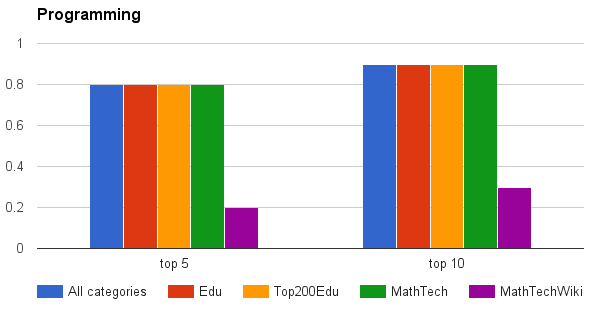
\includegraphics[width=\textwidth]{charts/p}
\label{fig:p}
\end{figure}

\begin{figure}[h] 
\caption{Precision score when the keyword \textit{Heuristic} is used as a search phrase, with the different white lists applied.}
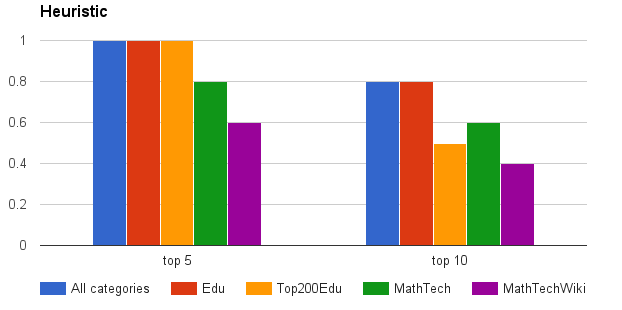
\includegraphics[width=\textwidth]{charts/h}
\label{fig:h}
\end{figure}

\begin{figure}[h] 
\caption{Precision score when the keyword \textit{Algebra} is used as a search phrase, with the different white lists applied.}
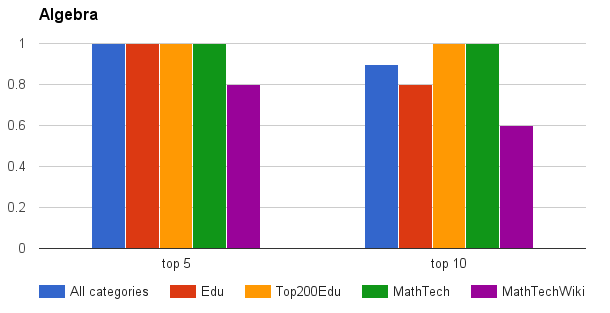
\includegraphics[width=\textwidth]{charts/a}
\label{fig:a}
\end{figure}

\begin{figure}[h] 
\caption{Precision score when the keyword \textit{Game Theory} is used as a search phrase, with the different white lists applied.}
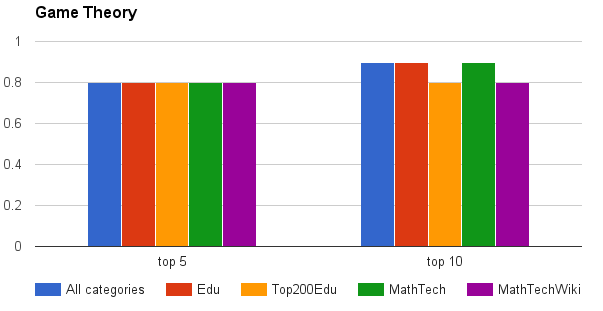
\includegraphics[width=\textwidth]{charts/gt}
\label{fig:gt}
\end{figure}

\begin{figure}[h] 
\caption{Precision score when the keyword \textit{Fuzzy Logic} is used as a search phrase, with the different white lists applied.}
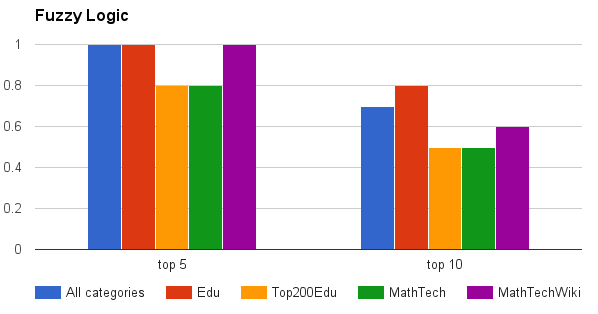
\includegraphics[width=\textwidth]{charts/fl}
\label{fig:fl}
\end{figure}

\begin{figure}[h] 
\caption{Precision score when the keyword \textit{Java} is used as a search phrase, with the different white lists applied.}
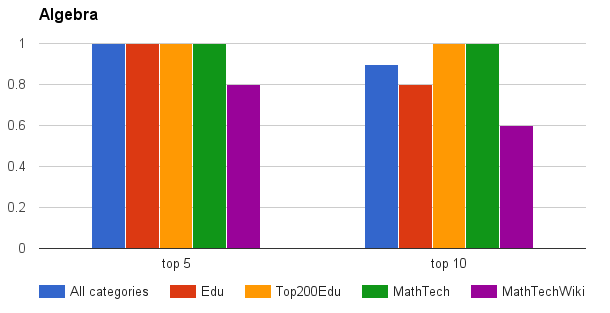
\includegraphics[width=\textwidth]{charts/a}
\label{fig:a}
\end{figure}

\begin{figure}[h] 
\caption{Precision score when the keyword \textit{Bayes Network} is used as a search phrase, with the different white lists applied.}
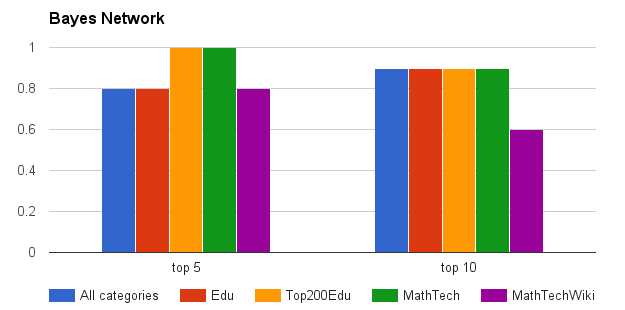
\includegraphics[width=\textwidth]{charts/bn}
\label{fig:bn}
\end{figure}

\begin{figure}[h] 
\caption{Precision score when the keyword \textit{Derivation} is used as a search phrase, with the different white lists applied.}
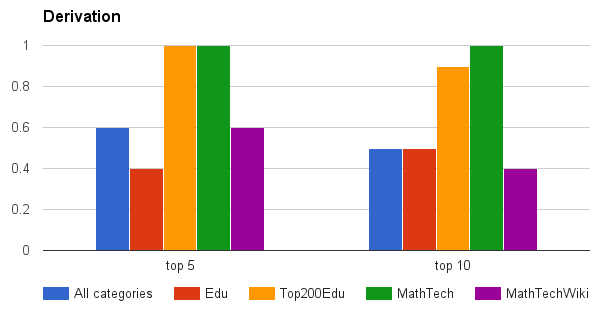
\includegraphics[width=\textwidth]{charts/d}
\label{fig:d}
\end{figure}

\begin{figure}[h] 
\caption{Precision score when the keyword \textit{Chain Rule} is used as a search phrase, with the different white lists applied.}
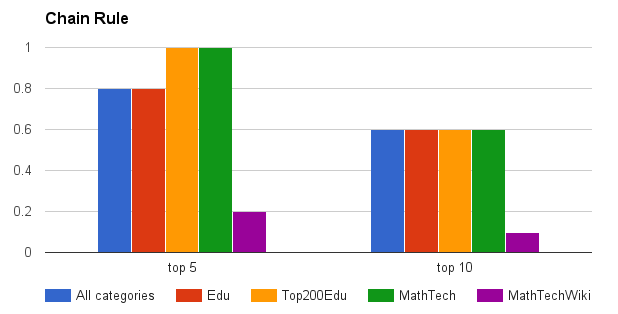
\includegraphics[width=\textwidth]{charts/cr}
\label{fig:cr}
\end{figure}

\begin{figure}[h] 
\caption{Precision score when the keyword \textit{Prisoners Dilemma} is used as a search phrase, with the different white lists applied.}
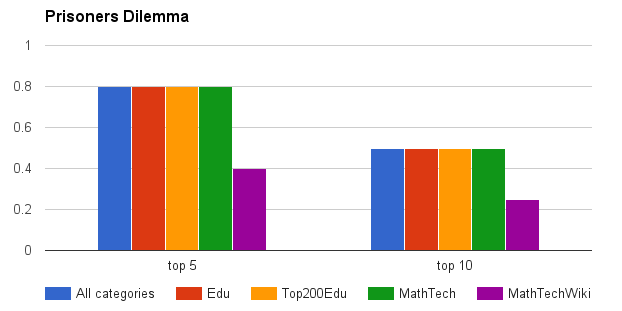
\includegraphics[width=\textwidth]{charts/pd}
\label{fig:pd}
\end{figure}

\begin{figure}[h] 
\caption{Precision score when the keyword \textit{Nash Equilibrium} is used as a search phrase, with the different white lists applied.}
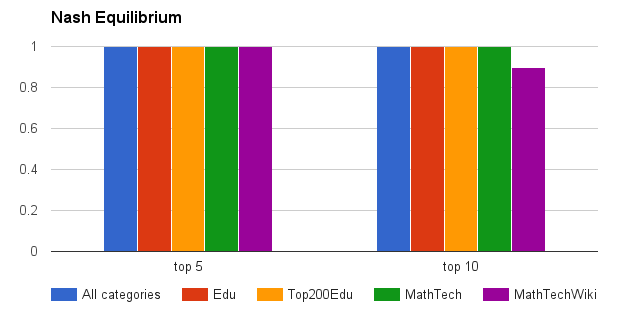
\includegraphics[width=\textwidth]{charts/ne}
\label{fig:ne}
\end{figure}

\begin{figure}[h] 
\caption{Precision score when the keyword \textit{Cartesian Product} is used as a search phrase, with the different white lists applied.}
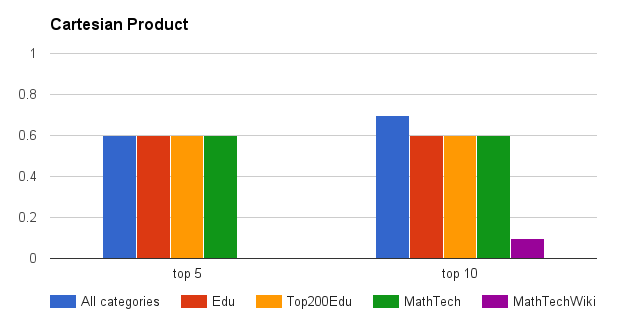
\includegraphics[width=\textwidth]{charts/cp}
\label{fig:cp}
\end{figure}

\begin{figure}[h] 
\caption{Precision score when the keyword \textit{Parrondos Paradox} is used as a search phrase, with the different white lists applied.}
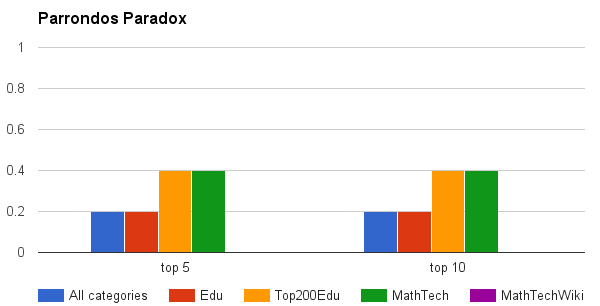
\includegraphics[width=\textwidth]{charts/pp}
\label{fig:pp}
\end{figure}

\begin{figure}[h] 
\caption{Precision score when the keyword \textit{Zero Sum} is used as a search phrase, with the different white lists applied.}
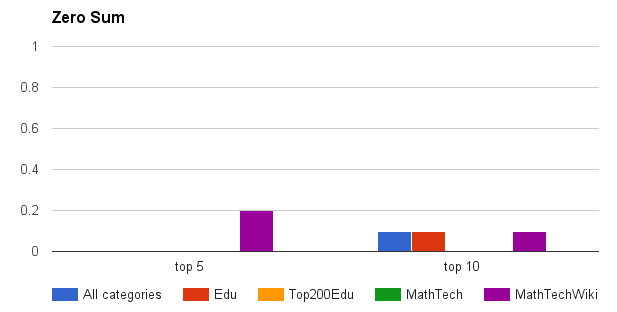
\includegraphics[width=\textwidth]{charts/zs}
\label{fig:zs}
\end{figure}


